\documentclass[5p,times]{elsarticle}

% YTT
\usepackage{tikz}
\usetikzlibrary{arrows.meta,positioning,calc}
\usepackage{xcolor}

\usepackage[UTF8,scheme=plain]{ctex}

\newif\ifshowcomments
\showcommentstrue

\newcommand{\cncomment}[1]{%
  \ifshowcomments
    \textcolor{red}{\textbf{【作者批注：#1】}%
  }\fi
}

\usepackage[normalem]{ulem}

\newcommand{\delcomment}[2]{%
  \textcolor{red}{\sout{#1}}%
  \textcolor{red}{【#2】}%
}

\usepackage{amsmath,amsfonts,amssymb}
\usepackage{algorithm}
\usepackage{algorithmic}
\usepackage{placeins}
\usepackage{array}
\usepackage{subfig}
\usepackage{textcomp}
\usepackage{url}
\usepackage{graphicx}
\usepackage{booktabs}
\usepackage{makecell}
\usepackage{multirow}
\usepackage{adjustbox}
\usepackage{tabularx}
\usepackage{amsthm}

% Compact, flexible float placement for the journal's two-column layout.
\setcounter{topnumber}{4}
\setcounter{dbltopnumber}{4}
\renewcommand{\topfraction}{0.95}
\renewcommand{\dbltopfraction}{0.95}
\renewcommand{\textfraction}{0.05}
\renewcommand{\floatpagefraction}{0.85}
\renewcommand{\dblfloatpagefraction}{0.85}
\setlength{\textfloatsep}{8pt plus 2pt minus 2pt}
\setlength{\dbltextfloatsep}{8pt plus 2pt minus 2pt}
\setlength{\emergencystretch}{2em}
\urlstyle{same}

\graphicspath{{figures/}{figures_en/}}

\journal{Future Generation Computer Systems-The International Journal of eScience}

\theoremstyle{plain}
\newtheorem{theorem}{Theorem}
\newtheorem{lemma}[theorem]{Lemma}
\newtheorem{proposition}[theorem]{Proposition}
\newtheorem{corollary}[theorem]{Corollary}
\newtheorem{assumption}[theorem]{Assumption}

\theoremstyle{definition}
\newtheorem{definition}[theorem]{Definition}

\theoremstyle{remark}
\newtheorem{remark}[theorem]{Remark}

\newcommand{\tabref}[1]{Table~\ref{#1}}
\newcommand{\figref}[1]{Fig.~\ref{#1}}
\newcommand{\secref}[1]{Section~\ref{#1}}
\newcommand{\equref}[1]{(\ref{#1})}

\makeatletter
\newenvironment{breakablealgorithm}
{%
  \par\addvspace{\intextsep}
  \refstepcounter{algorithm}%
  \hrule height 0.8pt depth 0pt
  \kern 2pt
  \renewcommand{\caption}[2][\relax]{%
    \noindent\textbf{\ALG@name~\thealgorithm}\ ##2\par
    \ifx\relax##1\relax
      \addcontentsline{loa}{algorithm}{\protect\numberline{\thealgorithm}##2}%
    \else
      \addcontentsline{loa}{algorithm}{\protect\numberline{\thealgorithm}##1}%
    \fi
    \kern 2pt
    \hrule height 0.8pt depth 0pt
    \kern 2pt
  }%
}
{%
  \kern 2pt
  \hrule height 0.8pt depth 0pt
  \par\addvspace{\intextsep}
}
\makeatother

\begin{document}

\begin{frontmatter}

\title{Dynamic Collaboration Mode Selection in Hierarchical Federated Learning}

\author[bupt1,bupt2,bupt3]{Tingting Yang}
\author[bupt1,bupt2,bupt3]{Wenbo Zhang}
\author[bupt1,bupt2,bupt3]{Shaohua Liu}
\author[bupt1,bupt2,bupt3]{Lihua Zhang}
\author[bupt1,bupt2,bupt3]{Xinyuan Lin}
\author[bupt1,bupt2,bupt3]{Qian Liu}

\affiliation[bupt1]{
    organization={School of Mathematical Sciences, Beijing University of Posts and Telecommunications},
    city={Beijing},
    country={China}
}

\affiliation[bupt2]{
    organization={State Key Laboratory of Information Photonics and Optical Communications (Beijing University of Posts and Telecommunications)},
    city={Beijing},
    country={China}
}

\affiliation[bupt3]{
    organization={Key Laboratory of Mathematics and Information Networks (Beijing University of Posts and Telecommunications), Ministry of Education},
    city={Beijing},
    country={China}
}

\begin{abstract}
Hierarchical federated learning enables cloud-edge-end collaborative training, but fixed execution and aggregation schemes are insufficient to adapt to heterogeneous and dynamic conditions.
To address this challenge, a dynamic collaboration reconfiguration framework is proposed.
The framework selects collaboration modes according to the current system state and considers execution paths and aggregation strategies.
A historical update deviation model is developed
to estimate the Cloud update under different
collaboration mode distributions. The estimated
deviation and system latency are jointly considered
in the multiobjective optimization.
The estimated learning error and system latency are jointly considered as optimization objectives.
Feasible collaboration profiles are filtered by Pareto dominance and selected using the Chebyshev ideal point criterion.
Experiments on CIFAR-10 with ResNet-18 and Fashion-MNIST with LeNet-5 evaluate dynamic collaboration under heterogeneous resource and data conditions.
\end{abstract}

\begin{keyword} 
Internet of Things \sep hierarchical federated learning \sep cloud-edge-end collaboration \sep dynamic collaboration reconfiguration \sep differential privacy \sep device heterogeneity 
\end{keyword}

\end{frontmatter}
\section{Introduction}
\label{sec:introduction}
Federated learning (FL) enables multiple end devices to collaboratively train a shared model without transferring raw data to a central server~\cite{fedavg,ZHAO2026108518}. In AIoT systems, however, participating devices differ substantially in computational capability, memory capacity, communication quality, and local data distribution. Cloud-edge-end hierarchical federated learning (HFL) introduces edge servers between end devices and the cloud, providing intermediate aggregation and computation capabilities while reducing direct communication with the cloud~\cite{hfl,FLaTEC2026,yang2026hierarchical}.

Data and system heterogeneity can limit the effectiveness of fixed cloud-edge-end collaboration schemes across clients and training rounds. First, non-IID data can cause
local updates to drift in different directions and can degrade simple weighted
aggregation~\cite{fedavgm,fedprox,scaffold,khan2026accelerating,11214447}.
Second, system capabilities are heterogeneous. A weak end device may be unable
to handle the same workload or meet the same deadline as a stronger device,
whereas an edge or cloud server can undertake more computation~\cite{wang2019adaptivefl,FAN2026108249}.
A mode that suits one client in one round may be inefficient or infeasible
for the same client in another round, or for another client.

Existing work on HFL and cloud-edge-end collaboration has covered personalization,
resource allocation, wireless scheduling, heterogeneous models, and split
training~\cite{Personalizedhfl,JSJX202502007,dinh2021wirelessfl,BSBODP,mazloomi2025multiserver,SFETEC,11185336,YAO2026108495}.
These studies address different aspects of collaborative training. However, dynamically selecting execution and aggregation configurations according to individual client capabilities and changing system conditions remains an important problem.

Different collaboration modes have different
training and communication paths, which affect
system latency and Cloud updates. This paper
studies dynamic collaboration mode selection
under changing system conditions. Historical
Cloud updates are used to estimate the update
deviation of candidate mode distributions.
System latency and predicted update deviation
are jointly minimized while satisfying
privacy protection requirements.
\begin{itemize}
    \item A dynamic collaboration configuration space for cloud-edge-end federated learning is formulated, which enables execution and aggregation configurations to be selected according to current system conditions.

    \item A joint learning error model is constructed, which accounts for algorithmic deviation, aggregation deviation, and update perturbation. Together with system latency, the estimated learning error forms an optimization problem with two objectives under resource and protection constraints. Feasible configurations are compared using Pareto dominance, and the final configuration is selected using the Chebyshev ideal point criterion.

    \item
\end{itemize}

The remainder of this paper is organized as follows.
Section~\ref{sec:related_work} reviews related studies
on hierarchical federated learning and cloud-edge-end
collaboration.
Section~\ref{sec:model} introduces the system model
and formulates the latency and learning error objectives
under resource and privacy constraints.
Section~\ref{sec:algorithm} presents the proposed
dynamic collaboration selection algorithm.
Section~\ref{sec:experiment} evaluates its performance
through experiments.
Finally, Section~\ref{sec:conclusion} concludes the paper.

\section{Related Work}
\label{sec:related_work}
\subsection{HFL Under Heterogeneous Environments}
Existing HFL studies use edge servers for intermediate aggregation between end devices and the cloud~\cite{hfl}. Research on resource management in FL has investigated model pruning under bandwidth and device constraints~\cite{phfl}, adaptive local update frequency and model compression~\cite{xu2022adaptive,wang2019adaptivefl}, and wireless resource allocation~\cite{dinh2021wirelessfl}. Personalized FL and HFL studies have addressed data heterogeneity through client clustering, shared representations, and personalized model components~\cite{sattler2020clustered,collins2021exploiting,Personalizedhfl}. These studies address different aspects of heterogeneous federated training, including resource management, communication efficiency, and model personalization.

Beyond these aspects, heterogeneous device capabilities and changing system conditions can also affect how computation and aggregation are organized across the cloud, edge, and end layers. In this work, a collaboration configuration specifies where model computation is performed, how updates are transmitted, and where aggregation takes place. Different clients may use different configurations, and their configurations may be reconsidered as system conditions change. Since frequent reevaluation incurs computational overhead, we use a configurable selection period to determine when configurations are reevaluated. Related studies have also considered the cost of frequent changes in FL
scheduling decisions and reduced such overhead by maintaining selected client
sets over multiple rounds~\cite{CHEN2026112204,10757319}.

\subsection{Cloud-Edge-End Collaborative Federated Learning}

Cloud-edge-end collaborative FL distributes computation, communication, and aggregation tasks across end devices, edge servers, and the cloud. Different studies have explored how these tasks can be organized. FedAgg~\cite{BSBODP} employs bridge samples and online distillation to support collaboration among models of different sizes across the three layers. SFETEC~\cite{SFETEC} investigates split federated learning in Thing Edge Cloud environments, allowing model computation to be distributed across layers. Related task offloading research has also considered federated learning, privacy protection, and task efficiency in cloud-edge-end systems~\cite{dong2026privacyoffloading}. While these studies investigate different collaborative mechanisms, this work focuses on selecting feasible execution and aggregation configurations for individual clients under changing system conditions.

Task migration in mobile edge computing provides a related perspective on adapting execution placement to changing system conditions. Zhang and Zheng~\cite{ZHANG2019111} investigate task migration decisions under user mobility, while Zhu et al.~\cite{ZHU2024303} study load aware task migration for balancing workloads across edge nodes. Although task migration differs from federated learning collaboration reconfiguration, these studies illustrate the importance of adapting execution placement to system conditions.


\subsection{Privacy Preserving HFL}
Model parameters, gradients, and intermediate representations in federated
training may leak information about private data~\cite{zhu2019dlg}.
Differential privacy (DP) and homomorphic encryption (HE) are widely used
privacy protection techniques in FL~\cite{dwork2006calibrating,cheon2017ckks}.
For HFL, group local DP provides personalized privacy through sampling,
randomized response, and shuffling~\cite{GLDP}.
Adaptive DP FL studies have explored dynamic privacy budget allocation,
adaptive clipping, and client selection for adjusting privacy protection
during training~\cite{xu2025adpfl}.
Other HFL studies combine DP based protection and CKKS based HE for privacy
preserved data sharing scenarios~\cite{PPHFL}.
Related fog FL studies combine hierarchical aggregation, personalization, and DP
for IoT intrusion detection~\cite{islam2025pphffl}.
These studies mainly focus on the security guarantee, budget allocation, or
accuracy degradation of a particular privacy mechanism.
These studies mainly focus on the design, analysis, or adaptation of individual
privacy mechanisms. In this work, privacy requirements are considered jointly
with execution and aggregation configuration selection in cloud-edge-end
federated learning.

This paper jointly considers execution, aggregation, and protection
configuration in federated learning.
Existing categories optimize selected resources, training steps, or privacy
parameters within a prescribed collaboration structure. The proposed collaboration space enables different execution locations,
aggregation paths, transmitted objects, and privacy mechanisms to be compared
within one feasible decision model.
\section{Model Construction}
\label{sec:model}
\subsection{Collaborative Mode and Transmission Modeling}
\label{sec:link_model}
We consider a three-tier federated learning system
consisting of \(N\) clients, a set of edge servers,
and a central cloud server. Each client \(i\) is
associated with an edge server \(e(i)\). At round
\(t\), the system assigns a collaboration mode
\(h_i^t\in\mathcal H\) to each participating client,
allowing training and aggregation to be organized
across different tiers.

\textbf{Collaboration modes.}
Three collaboration modes are considered in the 
cloud-edge-end architecture, which are distinguished 
by their aggregation paths and client-side synchronization 
requirements.

In Edge-based Federated Learning ($FL_E$), 
clients perform local training and submit their updates 
to the Edge for aggregation. The aggregated Edge update 
is then asynchronously propagated to the Cloud, without 
requiring clients to wait for Cloud-side aggregation. In 
Edge--Cloud Federated Learning ($FL_{EC}$), a group of 
clients associated with the same Edge participates in a 
multi-stage collaborative process. The Edge performs $E_B$ 
processing stages before submitting a single final joint 
update to the Cloud for global aggregation. In Cloud-based 
Federated Learning ($FL_C$), clients directly submit their 
locally trained updates to the Cloud for aggregation without 
intermediate Edge aggregation.

Let \(L\), \(E\), and \(C\) denote the Local, Edge,
and Cloud tiers, respectively. The three candidate
collaboration modes are defined as
\begin{equation}
\mathcal H =
\{\mathrm{FL_E},\mathrm{FL_{EC}},\mathrm{FL_C}\}.
\label{eq:three_modes}
\end{equation}
In all three modes, raw training data remain on
the client. Local model updates or Edge-aggregated
updates are transmitted according to the selected
collaboration mode.


\subsubsection{Collaborative Training Blocks and Mode Flows}

Let \(L_B\) denote the number of local training
steps in each block, and let \(T_L(L_B)\) represent
the corresponding local training process followed
by model update generation.
During local training, 
gradients computed for each example are clipped, 
and Gaussian noise is added to the clipped gradients using differentially private stochastic gradient descent.
Let \(A_E\) and \(A_C\)
denote aggregation at the Edge and Cloud,
respectively.
For the \(FL_{EC}\) mode, \(E_B\) denotes
the number of Edge processing and aggregation
stages. At each stage, clients perform
\(L_B\) local training steps using the latest
model received from the Edge. After each
stage, the aggregated model is returned to
the clients for the next stage. The final
aggregated update is denoted by
\(\Delta_e^{(E_B)}\).
\begin{equation}
\begin{aligned}
\mathrm{FL_E}:~~&
T_L(L_B)
\xrightarrow{\mathrm{upd}} A_E
\xrightarrow{\mathrm{async\ upd}} A_C,\\
\mathrm{FL_{EC}}:~~&
T_L(L_B)
\xrightarrow{\mathrm{upd}} \Delta_e^{(E_B)}
\xrightarrow{\mathrm{upd}} A_C,\\
\mathrm{FL_C}:~~&
T_L(L_B)
\xrightarrow{\mathrm{upd}} A_C.
\end{aligned}
\label{eq:mode_flows}
\end{equation}
Here, The arrows indicate the direction of information flow.
 The label \(\mathrm{upd}\) indicates the transmission
of a model update to the next aggregation stage.
The label \(\mathrm{async\ upd}\) indicates
asynchronous update transmission without requiring
clients to wait for Cloud-side aggregation.

Figure~\ref{fig:eecblockflow} illustrates the
execution structures of the three collaboration
modes. Figures (a)--(c) show the execution and
aggregation processes of \(FL_E\), \(FL_{EC}\),
and \(FL_C\), respectively, while Fig.~(d)
compares the three modes from the perspective
of an individual client. Filled circles, hollow
circles, and hollow diamonds represent the
Local, Edge, and Cloud tiers, respectively.
Dashed arrows indicate model update transmissions,
and circular arrows represent aggregation
operations. Spring-like marks indicate that the transmitted
model updates contain noise introduced by
client-side DP-SGD during local training.

\begin{figure}[t]
\centering
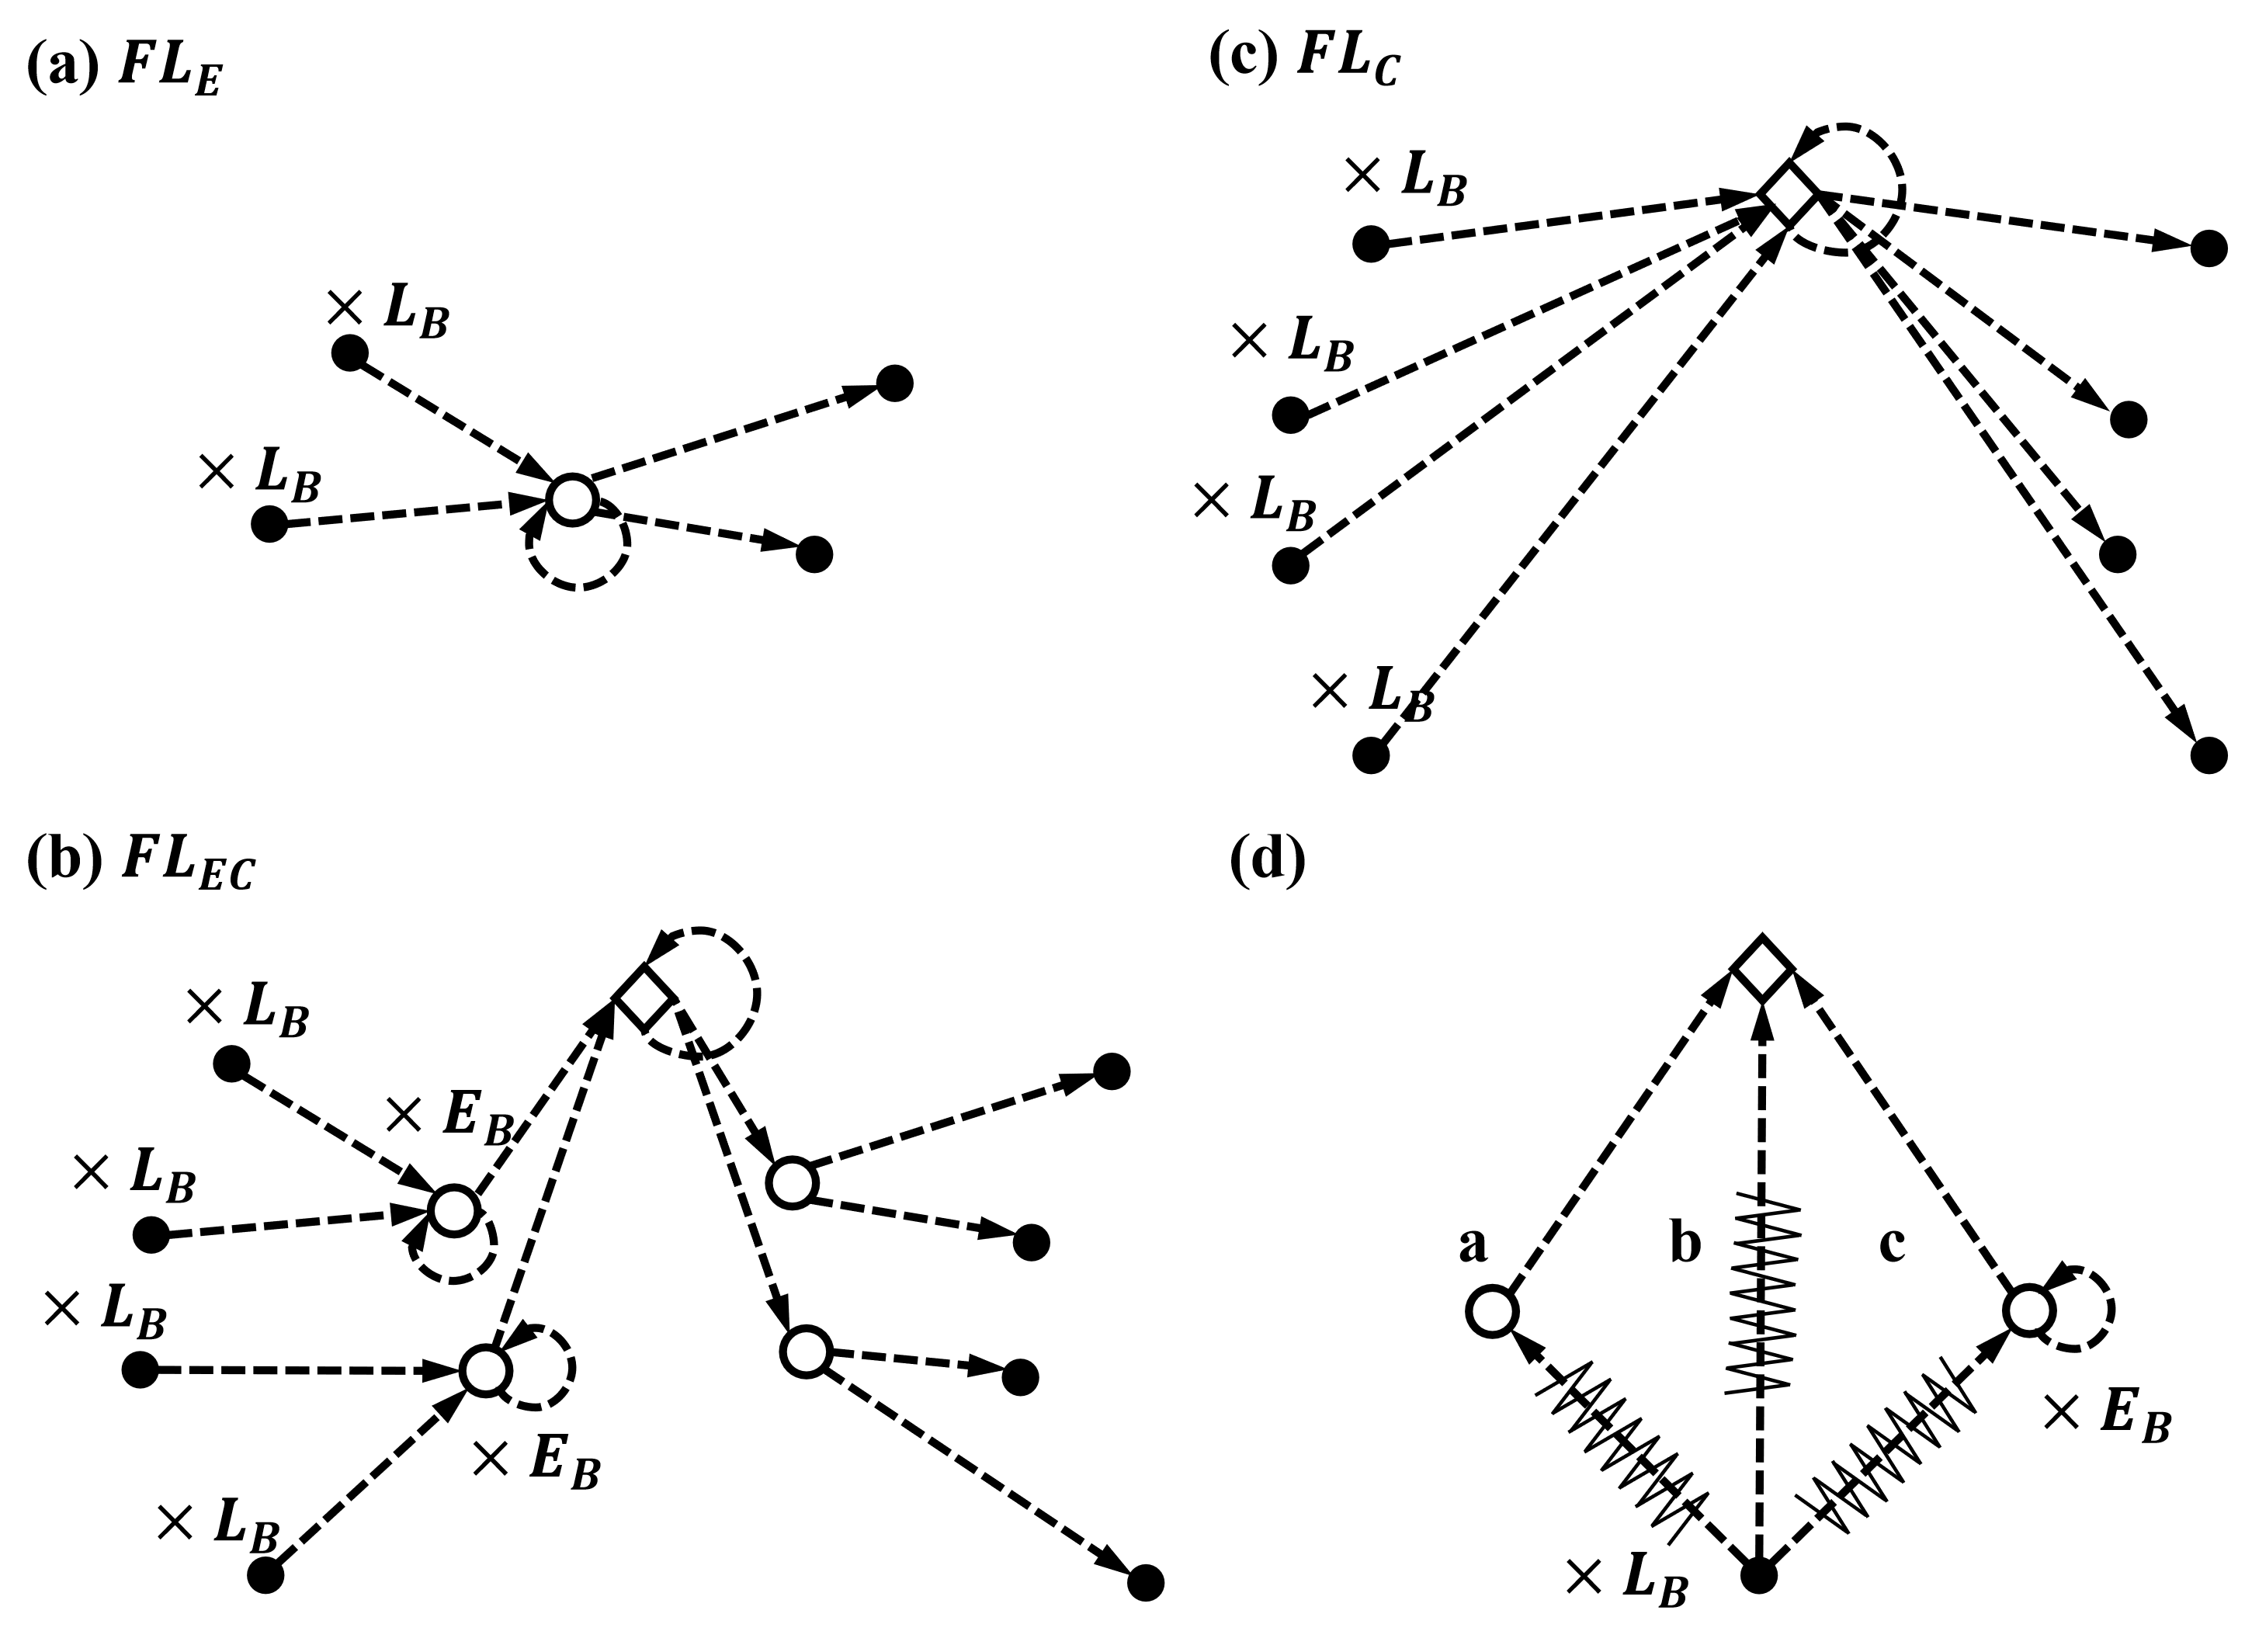
\includegraphics[width=\columnwidth]{eecblockflow.png}
\caption{Execution structures of the three collaboration modes in the cloud-edge-end architecture.}
\label{fig:eecblockflow}
\end{figure}

\subsection{Lifetime Privacy Accounting}
\label{sec:privacy_model}

Sample-level differential privacy~\cite{dwork2014the}
is enforced during local training through the
differentially private stochastic gradient descent
mechanism~\cite{abadi2016deep}, in which gradients
are clipped and Gaussian noise is added to the
clipped gradients. The resulting model updates
carry this noise when transmitted across tiers. For each client,
R\'enyi differential privacy (RDP)~\cite{mironov2017renyi}
is used to accumulate privacy loss across
training rounds. Let \(\mathcal A\) denote
the set of R\'enyi orders~\cite{vanerven2014renyi}. 
For a Gaussian
mechanism with noise multiplier \(\sigma\),
the RDP cost at order \(\alpha\in\mathcal A\)
is \(\rho(\alpha,\sigma)=\alpha/(2\sigma^2)\).

Let \(m_i^t\) denote the number of Gaussian
mechanisms applied to client \(i\) in round
\(t\), with corresponding noise multipliers
\(\sigma_{i,k}^t\).
The accumulated RDP cost can be calculated as
\begin{equation}
\Phi_i^{t+1}(\alpha)
=
\Phi_i^t(\alpha)
+
\sum_{k=1}^{m_i^t}
\rho(\alpha,\sigma_{i,k}^t).
\label{eq:rdp_update}
\end{equation}
For a given privacy parameter \(\delta\),
the corresponding privacy loss is
\begin{equation}
\epsilon_i^t
=
\min_{\alpha\in\mathcal A}
\left[
\Phi_i^t(\alpha)
+
\frac{\log(1/\delta)}{\alpha-1}
\right].
\label{eq:rdp_to_dp}
\end{equation}
Let \(\bar{\epsilon}\) denote the lifetime
privacy budget of each client. The accumulated
privacy loss must satisfy
\(\epsilon_i^t\leq\bar{\epsilon}\)
throughout training process.

For client \(i\) and candidate mode \(h\), let
\(N_i^t(h)\) denote the estimated number of Gaussian
mechanisms whose privacy costs are attributed to
client \(i\) over the remaining training rounds.
This estimate is determined by the planned local
training schedule and the protected releases
required by the selected mode. Let \(R\) denote
the total number of training rounds.

For \(N_i^t(h)>0\), the noise multiplier
\(\sigma_i^t(h)\) is calibrated to satisfy
\begin{equation}
\min_{\alpha\in\mathcal A}
\left[
\Phi_i^t(\alpha)
+
\frac{N_i^t(h)\alpha}
{2[\sigma_i^t(h)]^2}
+
\frac{\log(1/\delta)}{\alpha-1}
\right]
\leq\bar{\epsilon}.
\label{eq:noise_calibration}
\end{equation}
The smallest feasible multiplier is selected.
If calibration is infeasible, the candidate
mode is excluded. No calibration is required
when \(N_i^t(h)=0\).

Before execution, the planned privacy cost
is checked against the remaining budget.
The privacy ledger is updated using the
executed Gaussian mechanisms, and the resulting
RDP state is used for mode selection in
the next round.

\subsection{Joint Cost and Utility Modeling}
\label{sec:cost_utility_model}
Each collaboration mode is evaluated in terms
of resource feasibility, round latency, and
learning error, subject to the lifetime
privacy budget in Sec.~\ref{sec:privacy_model}.
\subsubsection{Path and Round Latency on a Common Timeline}

Figure~\ref{fig:system_timeline} provides two 
complementary views of collaboration latency. 
Fig.~\ref{fig:system_timeline}(a) illustrates the 
client-side execution and communication sequence 
of $FL_{EC}$, including the $E_B$ sequential Edge 
aggregation stages and the intermediate return 
transmissions from the Edge to the clients. 
After the final Edge aggregation stage, 
the resulting update is forwarded to the Cloud. 
Fig.~\ref{fig:system_timeline}(b) illustrates 
the system-level synchronization process for 
$FL_{EC}$ and $FL_C$. It shows how the final 
Edge updates and direct client updates determine 
the Cloud aggregation completion time, 
followed by the required return transmissions. 
For clarity, panel (b) uses $E_B=1$ as an 
illustrative example, while the latency 
formulation supports general $E_B$. 
The asynchronous Cloud upload in $FL_E$ 
is omitted from panel (b) because it does not 
impose a waiting dependency on the 
Cloud-synchronized round.
\begin{figure*}[t]
\centering
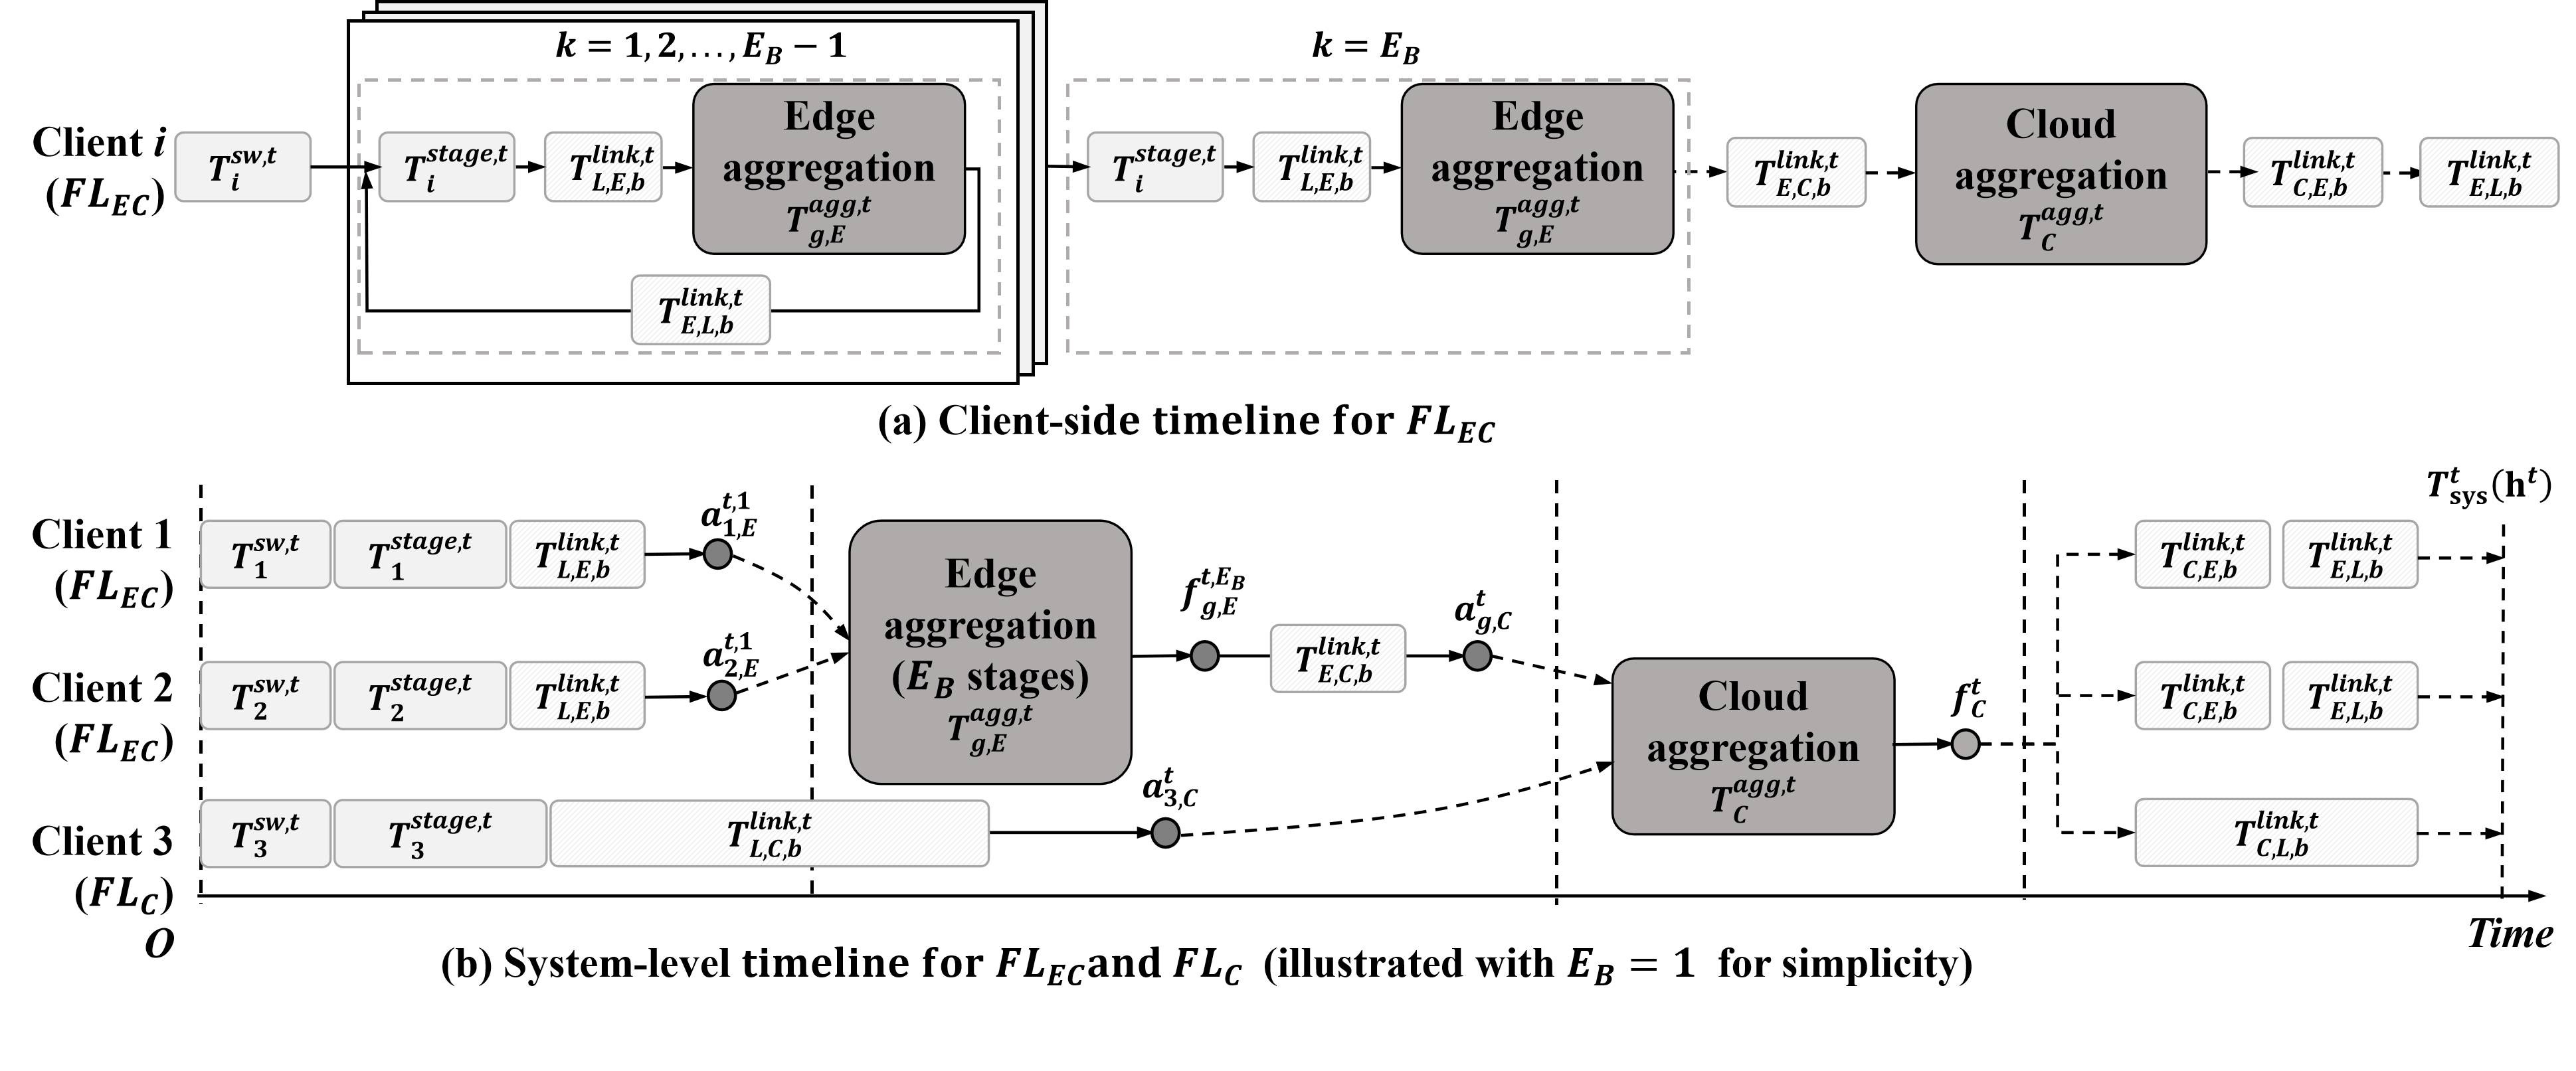
\includegraphics[width=\textwidth]{common_timeline.png}
\caption{Client-side and system-level latency timelines.
 (a) Client-side execution and communication path 
 for $FL_{EC}$, showing the $E_B$ sequential 
 Edge aggregation stages. 
 (b) System-level synchronization 
 timeline for $FL_{EC}$ and $FL_C$, 
 illustrated with $E_B=1$ for clarity. 
 Cloud aggregation waits for the final 
 $FL_{EC}$ Edge updates and direct $FL_C$ 
 client updates, followed by the required 
 return transmissions. The asynchronous 
 Cloud upload in $FL_E$ is omitted because 
 it does not delay the Cloud-synchronized round.}
\label{fig:system_timeline}
\end{figure*}

\textbf{Transmission latency.}
For a payload \(b\) transmitted from tier \(u\)
to tier \(v\), let \(S_{u,v,b}^t(h_i)\) denote
the original payload size under collaboration
mode \(h_i\). Let \(B_{i,u,v}^t\) denote
the transmission rate of the link between
tiers \(u\) and \(v\) for client \(i\) in
round \(t\), and let \(D_{u,v}^{0}\) denote
the fixed transmission delay of this link.
\begin{equation}
T_{u,v,b}^{\mathrm{link},t}(h_i)
=
\frac{
\kappa\!\left(\pi_i^{t,h_i}(u,v,b)\right)
S_{u,v,b}^t(h_i)}
{B_{i,u,v}^t}
+
D_{u,v}^{0}
+
T_{u,v,b}^{\mathrm{priv},t}
\!\left(\pi_i^{t,h_i}(u,v,b)\right).
\label{eq:comm_latency}
\end{equation}
Here, \(\kappa(\cdot)\) denotes the payload
expansion factor, and
\(T_{u,v,b}^{\mathrm{priv},t}(\cdot)\)
denotes the protection processing time.
For unprotected transmissions,
\(\kappa(\mathrm{none})=1\) and
\(T_{u,v,b}^{\mathrm{priv},t}(\mathrm{none})=0\).


\textbf{Execution latency.}
Let \(\tau_{i,L}^t(h)\) denote the estimated
execution time per local training step for
client \(i\) under mode \(h\).
The execution latency is given by
\begin{equation}
T_i^{\mathrm{stage},t}(h)
=
L_B\tau_{i,L}^t(h),
\quad
h\in\{FL_E,FL_{EC},FL_C\}.
\label{eq:execution_latency}
\end{equation}
Transmission and aggregation delays are
accounted for separately.

\textbf{Reconfiguration latency.}
Switching collaboration modes may require
reconfiguring the communication and aggregation
paths. We model the resulting reconfiguration
delay as
\begin{equation}
T_i^{\mathrm{sw},t}
=
\eta_h \mathbb{I}(h_i^t\neq h_i^{t-1}),
\label{eq:switching_cost}
\end{equation}
where \(\eta_h\) denotes the mode switching
overhead and \(\mathbb{I}(\cdot)\) is the
indicator function.

\textbf{Path arrival and aggregation.}
For each candidate mode \(h_i\), the mode flow
determines the sequence of execution stages
and payload transmissions leading to the
relevant aggregation point.
We calculate update arrival times by
following this sequence and accounting for
execution, transmission, and reconfiguration
delays in their order of occurrence.
Let \(a_{i,E}^{t,k}(h)\) denote the arrival time
of client \(i\)'s update at Edge stage \(k\)
under collaboration mode \(h\). Let \(a_{i,C}^t\)
denote the arrival time of client \(i\)'s update
at the Cloud under \(FL_C\).

Given a mode distribution
$\mathbf h^t=(h_1^t,\ldots,h_N^t)$,
clients are grouped by their associated Edge
and selected mode. Let
\begin{equation}
\mathcal G_{g,m}^t
=\{i\mid e(i)=g,\ h_i^t=m\},
\quad m\in\{FL_E,FL_{EC}\},
\label{eq:edge_mode_group}
\end{equation}
denote the clients assigned to mode $m$
at Edge $g$. Let \(k\) denote the
Edge aggregation stage index. For \(FL_E\),
only one Edge aggregation stage is performed,
whereas \(FL_{EC}\) consists of \(E_B\)
sequential Edge aggregation stages.

For \(h\in\{FL_E,FL_{EC}\}\), the update
arrival time at the first Edge stage is
\begin{equation}
a_{i,E}^{t,1}(h)
=
T_i^{\mathrm{sw},t}
+
T_i^{\mathrm{stage},t}(h)
+
T_{L,E,b}^{\mathrm{link},t}(h).
\end{equation}

For a nonempty Edge group
$\mathcal G_{g,m}^t$, the completion time
of aggregation stage $k$ is
\begin{equation}
f_{g,E}^{t,k}(m)
=
\max_{i\in\mathcal G_{g,m}^t}
a_{i,E}^{t,k}(m)
+
T_{g,E}^{\mathrm{agg},t},
\label{eq:edge_agg_finish}
\end{equation}
where $k=1$ for $FL_E$ and
$k=1,\ldots,E_B$ for $FL_{EC}$.
Updates arriving earlier remain buffered
until all required updates in the same
aggregation group have arrived.

For \(FL_{EC}\), each subsequent Edge stage
starts after the aggregated model from the
previous stage has been returned to the
clients. The clients then perform another
local training block and transmit their
updates to the Edge. Thus, for
\(k=1,\ldots,E_B-1\), the update arrival
time at the next stage is
\begin{equation}
\begin{aligned}
a_{i,E}^{t,k+1}(FL_{EC})
={}&f_{g,E}^{t,k}(FL_{EC})
+T_{E,L,b}^{\mathrm{link},t}(FL_{EC})\\
&+T_i^{\mathrm{stage},t}(FL_{EC})
+T_{L,E,b}^{\mathrm{link},t}(FL_{EC}).
\end{aligned}
\end{equation}

For \(FL_E\), the aggregated Edge update is
forwarded to the Cloud asynchronously after
the single Edge aggregation stage. This
transmission does not require clients to wait
for Cloud aggregation and is excluded from
the Cloud synchronization latency.

For \(FL_{EC}\), the final Edge update is
forwarded to the Cloud after the \(E_B\)-th
Edge aggregation stage. Its arrival time is
\begin{equation}
a_{g,C}^t
=
f_{g,E}^{t,E_B}(FL_{EC})
+
T_{E,C,b}^{\mathrm{link},t}.
\end{equation}

For \(FL_C\), clients transmit their updates
directly to the Cloud. The arrival time of
client \(i\)'s update is
\begin{equation}
a_{i,C}^t
=
T_i^{\mathrm{sw},t}
+
T_i^{\mathrm{stage},t}(FL_C)
+
T_{L,C,b}^{\mathrm{link},t}(FL_C).
\end{equation}

Cloud aggregation waits for the direct client
updates from $FL_C$ and the final Edge updates
from $FL_{EC}$. 
Let $\mathcal G_{EC}^t
=\{g\mid\mathcal G_{g,FL_{EC}}^t
\neq\emptyset\}$ denote the Edge servers
with active $FL_{EC}$ groups. The Cloud aggregation
completion time is
\begin{equation}
\begin{aligned}
f_C^t
={}&
\max\Bigg\{
\max_{i\in\mathcal D_C^t} a_{i,C}^t,\,
\max_{g\in\mathcal G_{EC}^t} a_{g,C}^t
\Bigg\}\\
&+T_C^{\mathrm{agg},t},
\label{eq:cloud_agg_finish}
\end{aligned}
\end{equation}
where $\mathcal D_C^t$ denotes the set of
$FL_C$ clients. The asynchronous uploads
of $FL_E$ do not affect the Cloud
synchronization time.

The system round latency is measured with
respect to the Cloud aggregation round.
Clients operating in \(FL_E\) are excluded
from this Cloud synchronization latency
because they do not wait for Cloud aggregation.
When required, return transmissions begin
after Cloud aggregation completes.
The system round latency is therefore
\begin{equation}
\begin{aligned}
T_{\mathrm{sys}}(\mathbf h^t)
={}&f_C^t+\max\Bigg\{
\max_{i\in\mathcal D_{EC}^t}
\Big(
T_{C,E,b}^{\mathrm{link},t}(h_i^t)
+
T_{E,L,b}^{\mathrm{link},t}(h_i^t)
\Big),\\
&\qquad
\max_{i\in\mathcal D_C^t}
T_{C,L,b}^{\mathrm{link},t}(h_i^t)
\Bigg\}.
\end{aligned}
\label{eq:system_round_latency}
\end{equation}

Here, $\mathcal D_{EC}^t=\{i\mid h_i^t=FL_{EC}\}$
and $\mathcal D_C^t=\{i\mid h_i^t=FL_C\}$
denote the corresponding client sets.
Clients operating in \(FL_E\) are excluded
from both sets because they do not wait for
Cloud aggregation.
Return delays are evaluated using
(\ref{eq:comm_latency}), with absent
return paths excluded from the maximum.

The client-side latency for each collaboration
mode is defined as
\begin{equation}
T_{i,\mathrm{client}}^t(h_i^t)
=
\begin{cases}
f_{g,E}^{t,1}(FL_E)
+T_{E,L,b}^{\mathrm{link},t}(h_i^t),
& h_i^t=FL_E,\\[4pt]
f_C^t
+T_{C,E,b}^{\mathrm{link},t}(h_i^t)
+T_{E,L,b}^{\mathrm{link},t}(h_i^t),
& h_i^t=FL_{EC},\\[4pt]
f_C^t
+T_{C,L,b}^{\mathrm{link},t}(h_i^t),
& h_i^t=FL_C.
\end{cases}
\label{eq:client_latency}
\end{equation}

\subsubsection{Historical Global Update Deviation Modeling}
\label{sec:learning_cost}

Different collaboration modes involve distinct
training and aggregation procedures, which may
result in different update characteristics.
The historical update deviations of each mode
are estimated from previous rounds and used
to evaluate the aggregate deviation signal
associated with each candidate mode distribution.

\textbf{Cloud aggregation and weights.}
For a candidate distribution
$\mathbf h^t=(h_1^t,\ldots,h_N^t)$,
clients connected to the same Edge and assigned
the same mode are grouped. Let
$\mathcal K^t(\mathbf h^t)$ denote the units
included in the current Cloud aggregation.
Each $FL_{EC}$ group contributes one final Edge update
after $E_B$ stages, while each $FL_C$ client
contributes its own update directly. 
For $FL_E$, each Edge group sends its
aggregated update to the Cloud asynchronously.
The update is included in the Cloud aggregation
that accepts it, without delaying the current
synchronization.

Figure~\ref{fig:client_mode_grouping} illustrates
how mode reassignment changes the grouping structure
and the resulting Cloud update units.
From Fig.~\ref{fig:client_mode_grouping}(a) to
Fig.~\ref{fig:client_mode_grouping}(b), client $l_2$
switches from $FL_{EC}$ to $FL_C$, while client $l_5$
switches from $FL_E$ to $FL_{EC}$.

For example, if the two configurations are applied
in consecutive rounds $t-1$ and $t$, respectively,
the set of Cloud update units changes from
\begin{equation}
\mathcal K^{t-1}(\mathbf h^{t-1})
=\{k_1,k_2,k_3,k_4,k_5,k_6\}
\end{equation}
to
\begin{equation}
\mathcal K^t(\mathbf h^t)
=\{k_1,k_2,k_3,k_4,k_5,k_6,k_7\}.
\end{equation}
Here, $k_i$ denotes the $i$th Cloud update unit
in the corresponding round.
The units are indexed separately in each round,
and their composition depends on the client
mode distribution.

\begin{figure}[t]
    \centering
    \subfloat[Before mode reassignment]{
        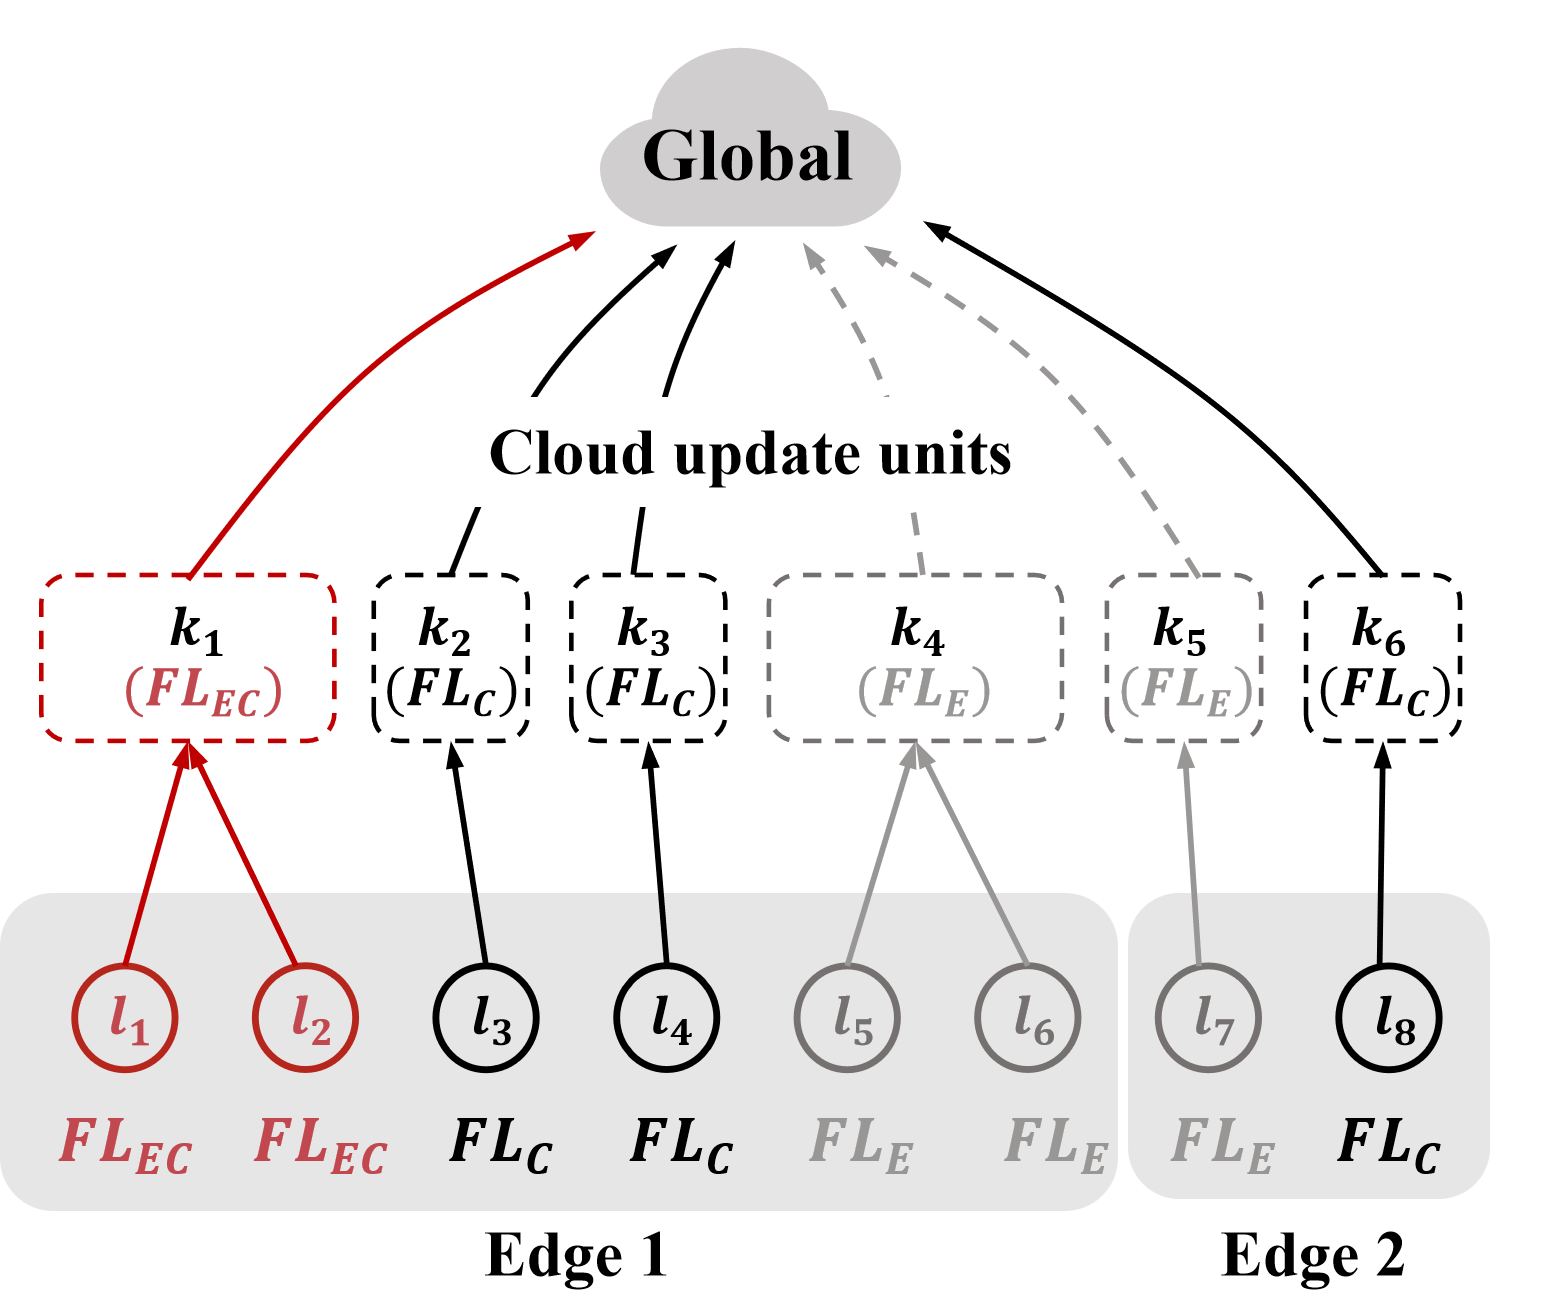
\includegraphics[width=0.90\columnwidth]
        {client_mode_grouping_a.png}
        \label{fig:client_mode_grouping_a}
    }

    \subfloat[After mode reassignment]{
        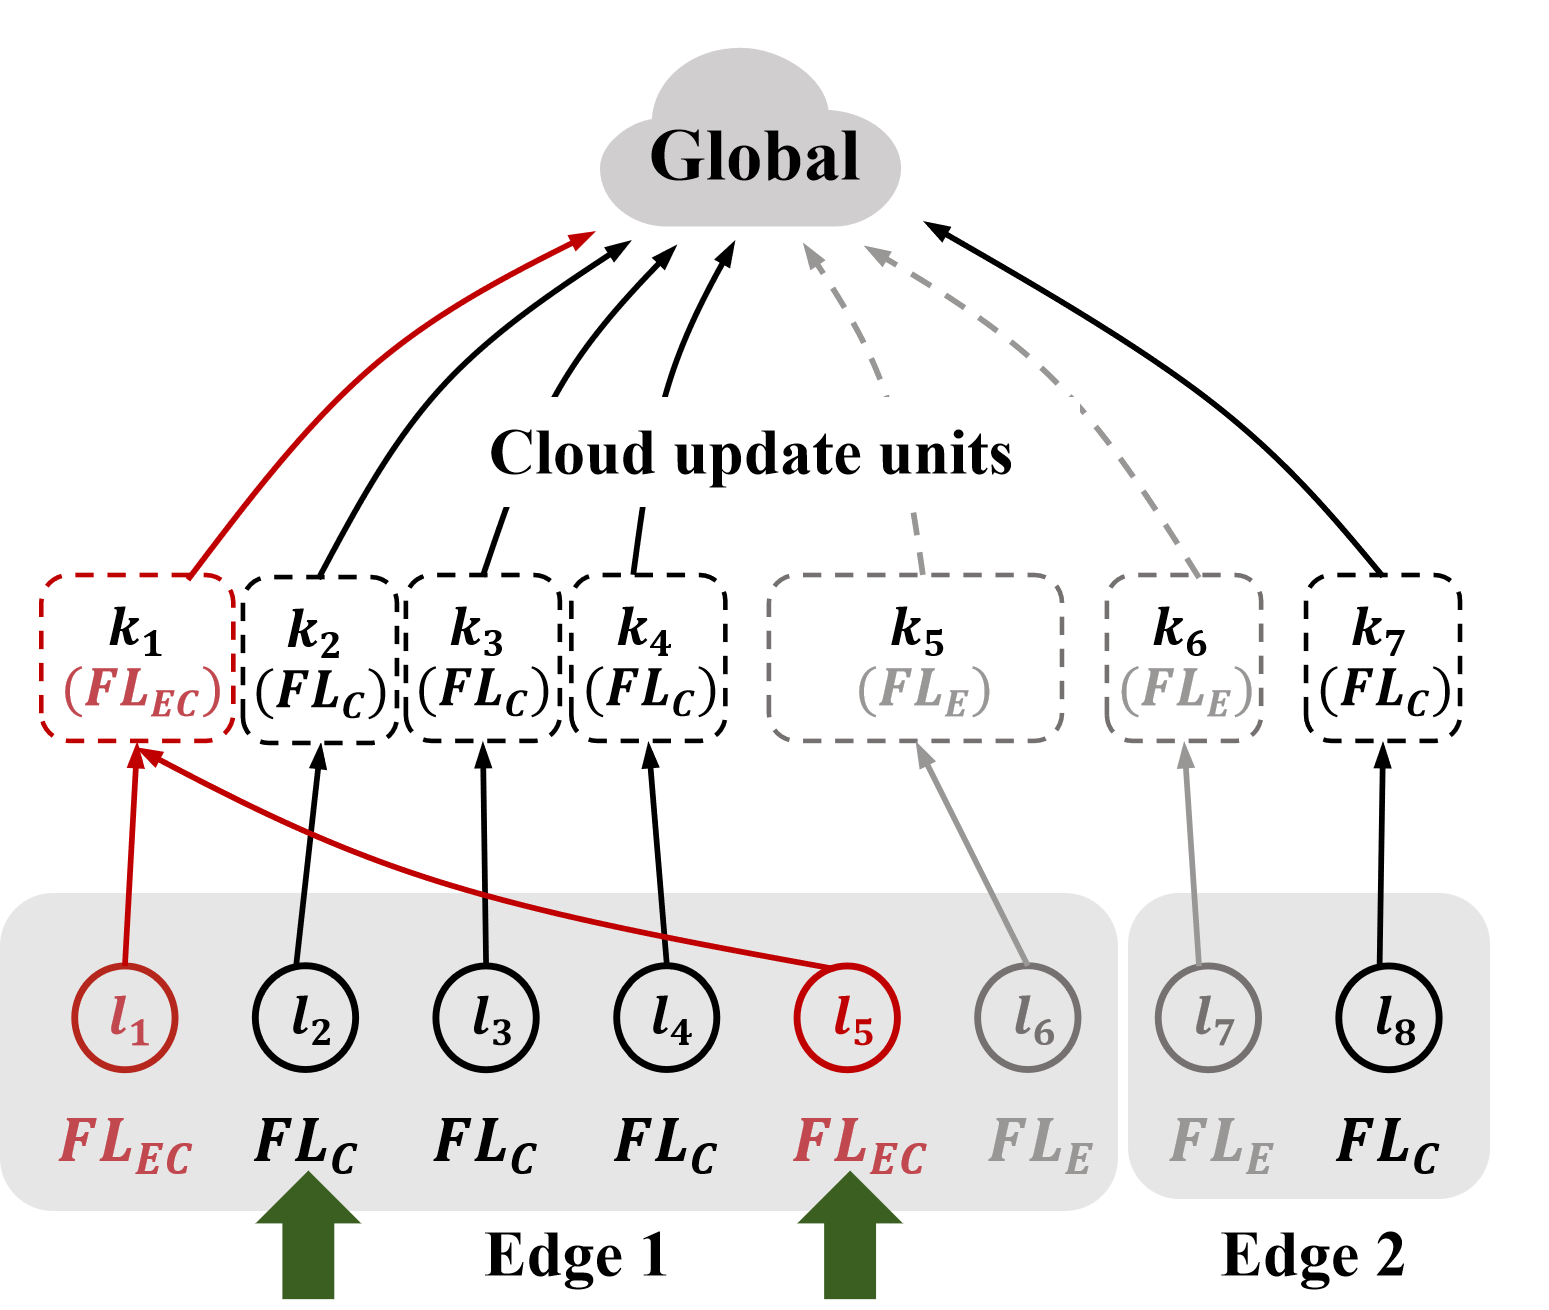
\includegraphics[width=0.90\columnwidth]
        {client_mode_grouping_b.png}
        \label{fig:client_mode_grouping_b}
    }

    \caption{Illustration of client grouping and Cloud
    update units under different mode distributions.
    From (a) to (b), client $l_2$ switches from
    $FL_{EC}$ to $FL_C$, while client $l_5$ switches
    from $FL_E$ to $FL_{EC}$. These changes alter
    the grouping structure and the resulting Cloud
    update units.}
    \label{fig:client_mode_grouping}
\end{figure}


Let $n_i$ denote the number of training samples
of client $i$, and let $\mathcal M_k^t$ denote
the clients represented by Cloud unit $k$.
The aggregation weight is calculated as
\begin{equation}
\begin{aligned}
N_k^t
&=\sum_{i\in\mathcal M_k^t}n_i,\\
I_k^t(\mathbf h^t)
&=\frac{N_k^t}
{\sum_{\ell\in\mathcal K^t(\mathbf h^t)}N_\ell^t}.
\end{aligned}
\label{eq:cloud_unit_weights}
\end{equation}

For example, in Fig.~\ref{fig:client_mode_grouping}(a),
unit $k_1$ represents clients $l_1$ and $l_2$,
with $N_{k_1}^{t-1}=n_1+n_2$.
In Fig.~\ref{fig:client_mode_grouping}(b),
unit $k_1$ instead represents clients $l_1$
and $l_5$, with $N_{k_1}^t=n_1+n_5$.
Meanwhile, client $l_2$ forms an individual
Cloud update unit $k_2$, with $N_{k_2}^t=n_2$.
The aggregation weights are determined by
these sample counts and the total samples
represented by the accepted Cloud units.

\textbf{Update deviation score.}
For each candidate mode distribution $\mathbf h^t$,
the Cloud units and their aggregation weights are determined.
The historical deviation contributions are aggregated
and combined with the global reference as follows:
\begin{equation}
\widehat U_C^t(\mathbf h^t)
=v_g^{t-1}
+\sum_{k\in\mathcal K^t(\mathbf h^t)}
I_k^t(\mathbf h^t)\widehat d_{m(k)}^t,
\label{eq:predicted_cloud_update}
\end{equation}
Here, $m(k)$ denotes the collaboration mode
of Cloud update unit $k$.
For example, in Fig.~\ref{fig:client_mode_grouping}(b),
$m(k_1)=FL_{EC}$ and $m(k_2)=FL_C$.
Their contributions to the aggregate deviation
are weighted by $I_{k_1}^t(\mathbf h^t)$
and $I_{k_2}^t(\mathbf h^t)$, respectively.
The update deviation score measures the normalized
squared magnitude of the aggregate historical
deviation contribution:
\begin{equation}
J^t(\mathbf h^t)
=\frac{\left\|\widehat U_C^t(\mathbf h^t)
-v_g^{t-1}\right\|_2^2}
{\left\|v_g^{t-1}\right\|_2^2+\varepsilon_J},
\quad\varepsilon_J>0.
\label{eq:j_learn_estimate}
\end{equation}
A larger $J^t(\mathbf h^t)$ indicates a stronger
aggregate historical deviation contribution
under the candidate mode distribution.
Therefore, larger values of $J^t(\mathbf h^t)$
are preferred to prioritize mode distributions
with more pronounced historical update
characteristics.
The system latency is also considered to
balance the historical deviation contribution
and the execution overhead.

\subsection{Finite Candidate Joint Selection}
\label{sec:global_optimization}

Let $P_j$ denote a candidate mode distribution,
where $j=0,\ldots,M-1$ and $M$ is the number
of candidate distributions considered.
Each candidate specifies the proportions
of clients assigned to $(FL_E,FL_{EC},FL_C)$,
which are used to construct client mode
assignments at each Edge.

Let $\mathcal F_{\mathrm{sys}}^t$ denote the set
of client mode distributions satisfying the
resource, privacy, and system admission
constraints in round $t$.
The feasible candidate set is defined as
\begin{equation}
\mathcal C^t
=
\left\{
P_j \mid
0\leq j<M,\;
P_j\in\mathcal F_{\mathrm{sys}}^t
\right\}.
\label{eq:feasible_candidates}
\end{equation}
The search complexity is $O(M)$,
as at most $M$ candidate distributions
are considered for joint utility maximization.

The candidate set can be extended by considering
additional mode distributions.
For experimental evaluation, five candidate
mode distributions are considered, with $M=5$.
Their proportions for $(FL_E,FL_{EC},FL_C)$
are specified as
\[
\begin{array}{ll}
P_0=(0.30,0.30,0.40), & P_1=(0.50,0.25,0.25),\\
P_2=(0.25,0.50,0.25), & P_3=(0.25,0.25,0.50),\\
P_4=(0.40,0.40,0.20). &
\end{array}
\]
For simplicity, the specified proportions
are applied separately to the clients
connected to each Edge.
For example, if an Edge serves ten clients,
candidate $P_0$ assigns three clients to
$FL_E$, three to $FL_{EC}$, and four to $FL_C$.
The number of clients assigned to each mode
is rounded to the nearest integer and adjusted
to match the total number of clients at each Edge.

For each feasible candidate $P_j\in\mathcal C^t$,
the corresponding client mode distribution
$\mathbf h^t$ is evaluated using
$J^t(\mathbf h^t)$ and
$T_{\mathrm{sys}}(\mathbf h^t)$.
All candidates are evaluated using the
historical statistics and system conditions
available in round $t$.

Since the two quantities have different scales,
their values are normalized among the feasible
candidates in each round.
Let $J_{\min}^t$ and $J_{\max}^t$ denote the
minimum and maximum values of $J^t$.
Similarly, $T_{\min}^t$ and $T_{\max}^t$
denote the minimum and maximum system latencies.

The joint utility is defined as
\begin{equation}
\begin{aligned}
U^t(\mathbf h^t;\lambda)
={}&\lambda
\frac{J^t(\mathbf h^t)-J_{\min}^t}
{J_{\max}^t-J_{\min}^t}\\
&+(1-\lambda)
\frac{T_{\max}^t-T_{\mathrm{sys}}(\mathbf h^t)}
{T_{\max}^t-T_{\min}^t},
\end{aligned}
\label{eq:joint_utility}
\end{equation}
where $0\leq\lambda\leq1$ controls the relative
importance of the historical deviation
contribution and system latency.
A normalized value of $0.5$ is used when
the corresponding maximum and minimum are equal.

A larger $J^t(\mathbf h^t)$ is preferred
to favor stronger historical aggregate
deviation contributions.
A smaller $T_{\mathrm{sys}}(\mathbf h^t)$
is preferred to reduce system execution time.
Both preferences are therefore represented
by larger normalized values in the joint utility.

The mode distribution is selected by
\begin{equation}
\mathbf h^{t,\ast}
\in
\arg\max_{\mathbf h^t\in\mathcal C^t}
U^t(\mathbf h^t;\lambda).
\label{eq:joint_selection}
\end{equation}
If multiple candidates achieve the same
maximum utility, the candidate with the
smallest index is selected.

\section{Algorithm}
\label{sec:algorithm}

Algorithm~\ref{alg:selection} presents the
dynamic collaboration mode selection procedure,
and the main symbols are summarized in
Table~\ref{tab:algorithm_notation}.
At each mode selection step, at most $M$
candidate distributions are evaluated
based on their feasibility, historical
deviation contribution, and system latency.
The candidate search complexity is $O(M)$
in terms of the number of candidate evaluations.

\begin{table}[t]
\centering
\caption{Notation Used in Algorithm~\ref{alg:selection}}
\label{tab:algorithm_notation}
\small
\setlength{\tabcolsep}{4pt}
\begin{tabular}{p{0.37\columnwidth}p{0.54\columnwidth}}
\hline
\textbf{Symbol} & \textbf{Description} \\
\hline
$M$ & Number of candidate mode distributions. \\
$P_j$ & Candidate mode distribution indexed by $j$. \\
$S_P$ & Mode selection period. \\
$\mathcal F_{\mathrm{sys}}^t$ &
Set of system feasible mode distributions. \\
$\mathcal C^t$ &
Set of feasible candidate distributions in round $t$. \\
$\mathbf h^{t,\ast}$ &
Selected mode distribution in round $t$. \\
$J^t(\mathbf h^t)$ &
Historical aggregate deviation contribution. \\
$T_{\mathrm{sys}}(\mathbf h^t)$ &
System latency under distribution $\mathbf h^t$. \\
$U^t(\mathbf h^t;\lambda)$ &
Joint utility for candidate selection. \\
\hline
\end{tabular}
\end{table}

\begin{breakablealgorithm}
\caption{Dynamic Collaboration Mode Selection}
\label{alg:selection}
\small
\begin{algorithmic}[1]
\REQUIRE Round $t$, candidate distributions
$\{P_j\}_{j=0}^{M-1}$,
strategy period $S_P$,
utility weight $\lambda$,
system state, privacy ledger,
and historical statistics
\ENSURE Selected mode distribution
$\mathbf h^{t,\ast}$ or \textsc{skip}

\IF{$t>1$,
$\operatorname{mod}(t-1,S_P)\neq0$,
and $\mathbf h^{t-1,\ast}
\in\mathcal F_{\mathrm{sys}}^t$}

    \STATE $\mathbf h^{t,\ast}
    \leftarrow\mathbf h^{t-1,\ast}$

\ELSE

    \STATE Construct $\mathcal C^t$
    using \eqref{eq:feasible_candidates}

    \IF{$\mathcal C^t=\emptyset$}
        \STATE \textbf{return} \textsc{skip}
    \ENDIF

    \STATE Freeze $v_g^{t-1}$ and
    $\{\widehat d_m^t\}_{m\in\mathcal H}$

    \FORALL{$\mathbf h^t\in\mathcal C^t$}

        \STATE Evaluate
        $J^t(\mathbf h^t)$
        using \eqref{eq:j_learn_estimate}

        \STATE Evaluate
        $T_{\mathrm{sys}}(\mathbf h^t)$
        using \eqref{eq:system_round_latency}

        \STATE Compute
        $U^t(\mathbf h^t;\lambda)$
        using \eqref{eq:joint_utility}

    \ENDFOR

    \STATE Select $\mathbf h^{t,\ast}$
    using \eqref{eq:joint_selection}

    \STATE Resolve utility ties
    by selecting the candidate
    with the smallest index $j$

\ENDIF

\STATE \textbf{return} $\mathbf h^{t,\ast}$

\end{algorithmic}
\end{breakablealgorithm}

\section{Experiments}
\label{sec:experiment}

This section evaluates the learning and system behavior of the finite
candidate selection mechanism.  The central question is whether
$U^t(\mathbf h^t;\lambda)$ can retain candidates with a strong
historical aggregate deviation contribution $J^t(\mathbf h^t)$ while
limiting the simulated system latency
$T_{\mathrm{sys}}(\mathbf h^t)$.  Test performance is always measured
after execution and is never used by the online selector.\cncomment{这句是防御性表达，可以直接说因为需要在线选择，所以使用可观测的指标}

\subsection{Experimental Setup}
\label{sec:exp_setup}

Table~\ref{tab:experimental_setup} summarizes the common configuration.

\textbf{Datasets and training configuration.}
Fashion MNIST supplies 60,000 training images and 10,000 test images.
The complete sets are used.  For each class, its training samples are
distributed among ten Edge servers according to a Dirichlet draw with
concentration 0.5.  The samples assigned to each Edge are then shuffled
and divided among its ten attached clients.  This procedure produces
label skew across Edges while preserving all training samples.
The model is a full parameter LeNet 5 network with two convolutional
layers and three fully connected layers.  Each experiment contains
100 clients, ten Edge servers, and 100 global rounds.  A local stage
uses two DP SGD steps with batch size 64 and learning rate 0.05.
$FL_{EC}$ executes three consecutive Edge stages, whereas $FL_E$ and
$FL_C$ execute one local stage per round.\cncomment{这里理解正确吗，本地epoch为1？}

\textbf{System heterogeneity.}
Each client receives a fixed computation factor sampled from
$\mathcal U(0.5,2.0)$\cncomment{没有解释}.  Its modeled local step duration equals
0.1 seconds multiplied by this factor, and its compute capacity equals
2.0 divided by the same factor.  Client memory is generated
independently as 32 MB multiplied by another draw from
$\mathcal U(0.5,2.0)$.  The feasibility thresholds are 1.0 compute
unit and 16 MB.\cncomment{这里写的太细了，其实我是100
\%接收的，因为这里不是我讨论的重点，所以没有必要写这么详细，我甚至没有讨论资源受限这篇论文}

Network rates are generated from reproducible traces.  In each round,
each client receives an independent multiplier from
$\mathcal U(0.75,1.25)$ for each logical path family.  The multiplier
scales base rates of 5.0 MB/s for Local to Edge, 2.2 MB/s for Local to
Cloud, and 8.0 MB/s for Edge to Cloud transmission.  

\textbf{Latency model.}\cncomment{有什么办法将时延模型一笔带过}

\textbf{Privacy configuration.}
Local optimization uses per example gradient clipping with
$C=1.0$ and one Gaussian mechanism per executed local step.  Under
replacement adjacency, the summed clipped gradient has sensitivity
$2C$, and the applied noise standard deviation is $2C\sigma$.
The per client RDP ledger does not claim sampling amplification.
Noise is calibrated against the remaining event budget.  The
preregistered worst path assigns every client to $FL_{EC}$ for all
100 rounds, which gives 600 mechanisms per client and
$\sigma=16.9793437$.  Its projected privacy expenditure is
$7.999999992$ at $\delta=10^{-5}$, below the declared limit
$\epsilon=8$.  Every reported run satisfies the same limit.\cncomment{这些参数虽然重要，但是如果直接写入配置表可能更好。因为前面已经花篇幅解释这些参数了，这里直接列表，写值，不需要长篇大论}\cncomment{这里最好补上一句通过J来反映包含DP的通信链路带来的影响可以规避正向讨论DP作用的难题，所以我们称之为满足隐私预算需求之下精度-时间的平衡}

\begin{table}[t]
\centering
\caption{FMNIST experimental configuration.\cncomment{这个表最好紧跟段落}}
\label{tab:experimental_setup}
\footnotesize
\setlength{\tabcolsep}{3.5pt}
\begin{tabularx}{\columnwidth}{@{}lX@{}}
\toprule
\textbf{Item} & \textbf{Setting} \\
\midrule
Data & 60,000 training and 10,000 test samples \\
Topology & 100 clients and 10 Edge servers \\
Partition & Edge label skew, Dirichlet concentration 0.5 \\
Training & 100 rounds, batch 64, learning rate 0.05 \\
Local work & 2 steps per stage; 3 stages for $FL_{EC}$ \\
Computation & 0.1 s base step; heterogeneity factor 2.0 \\
Network & 5.0, 2.2, and 8.0 MB/s; jitter 0.25 \cncomment{这是带宽还是什么，解释清楚}\\
Aggregation & 0.02 s per Edge stage; 0.04 s at Cloud \cncomment{不知道这样是否合理，我希望这个表格的配置出现方式更直白，因为左侧写的也并非专业用语}\\
Switching & $\eta_h=0.02$ s per changed client \\
Privacy & $C=1.0$, $\epsilon=8$, $\delta=10^{-5}$ \\
\bottomrule
\end{tabularx}
\end{table}

\subsection{Comparison Strategies and Evaluation Metrics}
\label{sec:exp_strategies_metrics}

\textbf{Comparison strategies.}
Five fixed candidates use $P_0,\ldots,P_4$ as defined in
Sec.~\ref{sec:global_optimization}.  Three pure baselines assign every
client to $FL_E$, $FL_{EC}$, or $FL_C$.  The greedy selectors maximize
$U^t(\mathbf h^t;\lambda)$ every round with
$\lambda\in\{0.25,0.50,0.75\}$.  Two stability variants use
$\lambda=0.50$: \cncomment{我不喜欢在论文中用冒号和分号}the hysteresis selector changes candidate only when
the utility improvement is greater than 0.05, and the periodic
selector permits a new decision every five rounds.  The objective
baselines select either the largest feasible $J^t(\mathbf h^t)$ or the
smallest feasible $T_{\mathrm{sys}}(\mathbf h^t)$.\cncomment{这里的用意是对比两种更保守的方式吗？如果是，请描述一下我们为什么设计这个，从后面看我甚至看不到这the periodic
selector是否存在优势，感觉没有}

All seven dynamic strategies execute $P_0$ during rounds 1 to 5 and
start online selection in round 6 from the same model, history,
privacy ledger, client state, and random state.  By contrast, fixed
$P_1$ to $P_4$ and the pure modes use their named configuration from
round 1. 

\textbf{Evaluation metrics.}
Test loss is the mean cross entropy over all 10,000 test samples, and
test accuracy is the corresponding fraction of correct predictions.\cncomment{这个test accuracy有必要解释吗？我也不清楚Test loss和test accuracy相比哪个更有说服力}
Cumulative system latency is the sum of recorded per round event
timeline durations in simulated seconds. \cncomment{有更体面的说法吗，我们一直在用simulated，如果非要说写为“仿真时间”}  Communication overhead is
the sum of transmitted payloads in MB.  Computation overhead is
reported as the number of executed local training steps because the
logs do not define a separate additive computation time outside the
critical path.

\cncomment{之后的内容主要是图需要需要大改，图改好内容才知道要围绕什么图说，还有就是不要一股脑把所有图都堆叠在一起，最好是能够跟段落距离不会太远.}
\cncomment{审稿人看到我们的实验之后无疑会发出疑问，复杂模型还适用吗，因此我们之后还要补上关于复杂数据集cifar10和resnet18的实验}

\subsection{Convergence Performance and Efficiency}
\label{sec:exp_convergence}
\label{sec:main_comparison}

Figure~\ref{fig:loss_vs_cumulative_latency} plots every raw test loss
against cumulative simulated system latency.  The two panels share
the same axes so that shorter traces are not visually stretched.
Pure $FL_E$ and pure $FL_C$ finish in 72.824 and 83.377 simulated
seconds, respectively, but both retain a final loss of 1.4016.
Pure $FL_{EC}$ requires 184.709 seconds and obtains the lowest final
loss, 1.1141.  This contrast exposes the cost of the additional local
and Edge stages rather than establishing that one mode is universally
preferable.

\begin{figure*}[t]
\centering
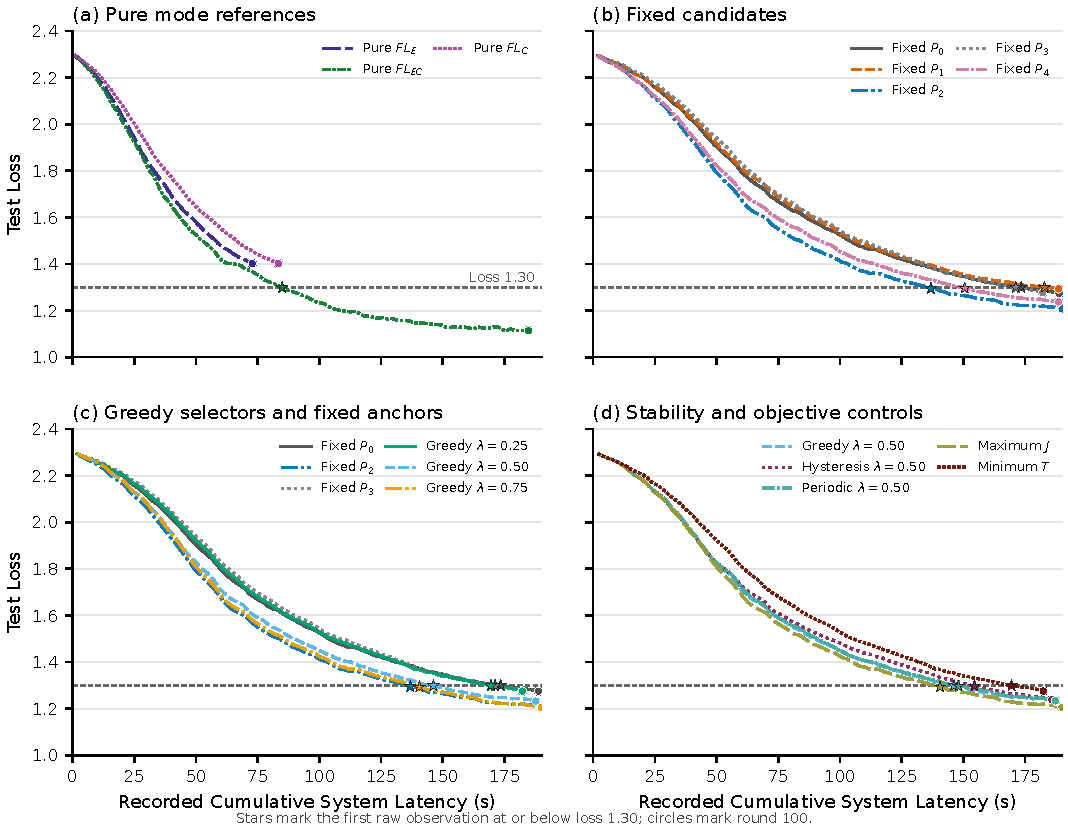
\includegraphics[width=0.98\textwidth]{experiment_loss_vs_cumulative_T.pdf}
\caption{Test loss versus cumulative simulated system latency for the
complete seed 42 matrix.  Panel (a) contains the fixed candidates and
pure mode baselines; panel (b) contains the dynamic selectors.  Each
curve contains the 100 raw round observations, and the marker denotes
the final round.  The horizontal coordinate is the accumulated event
timeline latency, not program execution time.\cncomment{这个图太大乱炖了，没有想好我们到底要说明什么问题，关于这个实验需要分开A.Pure FL\_E、Pure FL\_EC、PureFL\_C;B.Fixed+Dynamic,这样分组的目的是为了说明动态的作用（类似于消融），我们为了说明动比不动强，要说明三件事（其实是9件事，可以方便画在一个图上直观说明这九件事吗），1.1Greedy lambda=0.25比 Fixed P0在T方面强，1.2Greedy lambda=0.5比 Fixed P0在T和acc方面都强，1.3Greedy lambda=0.75比 Fixed P0在acc方面强2.1Greedy lambda=0.25比 Fixed P2在T方面强，2.2Greedy lambda=0.5比 Fixed P2在T方面强，2.3Greedy lambda=0.75比 Fixed P2在T方面强3.1Greedy lambda=0.25比 Fixed P3在acc/loss方面强，3.2Greedy lambda=0.5比 Fixed P3在acc/loss方面强，3.3Greedy lambda=0.75比 Fixed P3在acc/loss方面强，再解释一下我们为啥这么比较，应该先给出P0到P4的J/T图，这样就能展馆看到P2在J上绝对优势，P3在T上绝对优势，所以我们动态方法就可以取得两者之间的平衡方法，从J/T图可以看出帕累托前沿图P3、P0、P2构成的。但是我们再画一个acc/T的帕累托前沿图就可以发现Greedy lambda=0.25、Greedy lambda=0.5、Greedy lambda=0.75会在更前沿；C.Greedy lambda=0.5、Hysteresis lambda=0.5、Periodic lambda=0.5说实话我现在没看出后两者在loss图上有差异，但是在acc图上也许可以挖掘稳定性方面的差异，还有就是这个图应该将cumulative system latency vs test loss图上可以加几条辅助线帮我们看出不同线在达到统一水平loss时对应的时间，从而体现出效率的差异。}}
\label{fig:loss_vs_cumulative_latency}
\end{figure*}

Among candidate based methods, Greedy $\lambda=0.75$ reaches loss
1.2055 at 189.936 seconds, almost coinciding with Fixed $P_2$, which
reaches 1.2074 at 190.000 seconds.  The Maximum $J$ baseline is
identical to Greedy $\lambda=0.75$ in this run.  Greedy
$\lambda=0.50$, Periodic $\lambda=0.50$, and Hysteresis
$\lambda=0.50$ finish at losses 1.2322, 1.2333, and 1.2385 with
187.683, 187.211, and 185.852 seconds, respectively.  Greedy
$\lambda=0.25$ and Minimum $T$ both use 182.322 seconds and finish at
losses 1.2751 and 1.2753.  Thus increasing the weight assigned to $J$
moves the observed operating point toward lower loss and higher
system time, but the complete set also shows that pure $FL_{EC}$
achieves lower loss with a different and substantially larger
training workload.

Figure~\ref{fig:accuracy_round} gives the complementary accuracy
trajectory.  Loss and accuracy need not rank strategies identically.
For example, Fixed $P_1$ has higher final accuracy than Fixed $P_2$
(55.87\% versus 54.37\%) but higher final cross entropy
(1.2932 versus 1.2074).  Accuracy records only the winning class,
whereas cross entropy also reflects the assigned probabilities.  The
loss comparison therefore cannot be replaced by an accuracy ranking.

\begin{figure*}[t]
\centering
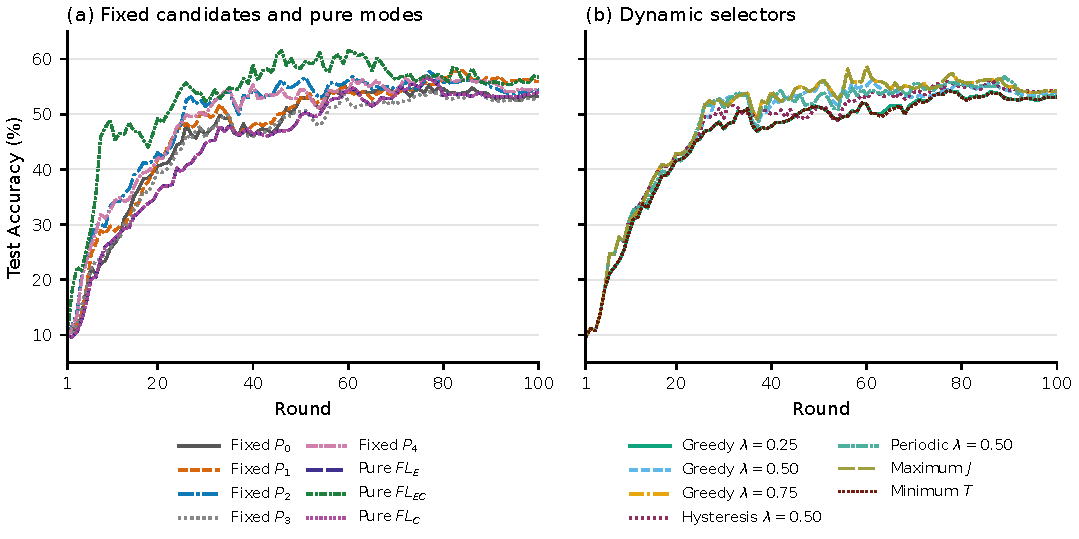
\includegraphics[width=0.98\textwidth]{experiment_accuracy_vs_round.pdf}
\caption{Raw test accuracy by training round for seed 42.  Both panels
use identical axes and the same strategy grouping as
Fig.~\ref{fig:loss_vs_cumulative_latency}.  Test measurements are
reported after each round and are not used by the selector.}
\label{fig:accuracy_round}
\end{figure*}

\subsection{Learning Performance and System Tradeoffs}
\label{sec:exp_tradeoffs}

Table~\ref{tab:final_tradeoffs} reports final learning performance and
the system work accumulated during the same 100 rounds.  Pure
$FL_{EC}$ produces the best loss and accuracy, but also executes
60,000 local steps and communicates 17,525.8 MB, the largest totals
in the table.  Greedy $\lambda=0.75$ reaches loss 1.2055 with
39,600 steps and 12,724.9 MB.  It is close to Fixed $P_2$ on all five
measures; both execute $P_2$ from round 6 onward, although only the
Greedy strategy uses the $P_0$ prefix.  At the low time end,
pure $FL_E$ is fastest, while pure $FL_C$ communicates the least.
Neither reaches the lower loss obtained by the strategies with more
$FL_{EC}$ work.

\begin{table*}[t]
\centering
\caption{Final learning performance and accumulated system cost for
the complete seed 42 matrix.  Local steps are the recorded computation
work, not wall clock time.  Mode changes count client reassignments.\cncomment{其实还可以加一个图，我想要再增加一个图分析一下loss，acc，local step 之间的相关性}}
\label{tab:final_tradeoffs}
\scriptsize
\setlength{\tabcolsep}{4.1pt}
\begin{tabular}{lrrrrrr}
\toprule
\textbf{Strategy} & \textbf{Final loss} & \textbf{Accuracy (\%)} &
\textbf{Cumulative $T$ (s)} & \textbf{Communication (MB)} &
\textbf{Local steps} & \textbf{Mode changes} \\
\midrule
Fixed $P_0$ & 1.2747 & 53.16 & 188.755 & 10,614.5 & 32,000 & 0 \\
Fixed $P_1$ & 1.2932 & 55.87 & 188.507 & 10,984.8 & 30,000 & 0 \\
Fixed $P_2$ & 1.2074 & 54.37 & 190.000 & 12,836.0 & 40,000 & 0 \\
Fixed $P_3$ & 1.2770 & 52.91 & 182.136 & 9,750.5 & 30,000 & 0 \\
Fixed $P_4$ & 1.2373 & 54.34 & 188.570 & 12,342.4 & 36,000 & 0 \\
\midrule
Greedy $\lambda=0.25$ & 1.2751 & 53.16 & 182.322 & 9,845.5 & 30,220 & 195 \\
Greedy $\lambda=0.50$ & 1.2322 & 54.00 & 187.683 & 12,038.7 & 37,040 & 1,558 \\
Greedy $\lambda=0.75$ & 1.2055 & 54.25 & 189.936 & 12,724.9 & 39,600 & 20 \\
Hysteresis $\lambda=0.50$ & 1.2385 & 54.26 & 185.852 & 11,298.2 & 34,640 & 649 \\
Periodic $\lambda=0.50$ & 1.2333 & 53.38 & 187.211 & 11,749.9 & 36,200 & 411 \\
Maximum $J$ & 1.2055 & 54.25 & 189.936 & 12,724.9 & 39,600 & 20 \\
Minimum $T$ & 1.2753 & 53.14 & 182.322 & 9,832.0 & 30,160 & 205 \\
\midrule
Pure $FL_E$ & 1.4016 & 53.93 & 72.824 & 10,121.1 & 20,000 & 0 \\
Pure $FL_{EC}$ & 1.1141 & 56.74 & 184.709 & 17,525.8 & 60,000 & 0 \\
Pure $FL_C$ & 1.4016 & 53.93 & 83.377 & 4,937.1 & 20,000 & 0 \\
\bottomrule
\end{tabular}
\end{table*}

All fifteen strategies reach 100 acknowledgments, zero pending update
units, and the same maximum privacy expenditure
$\epsilon_{\max}=7.999999992$.  The observed final loss and time
nondominated set, with lower values preferred for both coordinates,
contains Pure $FL_E$, Fixed $P_3$, Greedy $\lambda=0.25$, and Pure
$FL_{EC}$.  This set describes the recorded seed 42 operating points;
it is neither a statistical significance result nor the output of the
online selection algorithm.

\subsection{Joint Selection and Switching Behavior}
\label{sec:exp_joint_selection}
\label{sec:reconfiguration_behavior}

\textbf{Historical deviation and latency scores.}
To compare candidate scores under exactly the same information, the
round 6 decision is reconstructed from the state frozen after the
common fifth round.  All dynamic branches have the same model,
historical reference, privacy ledger, and trace at this point.
The five candidates have $(T_{\mathrm{sys}},J)$ values
$(1.8424,3.0543)$ for $P_0$, $(1.8486,2.9268)$ for $P_1$,
$(1.8486,4.5909)$ for $P_2$, $(1.7680,2.7985)$ for $P_3$, and
$(1.8486,3.7505)$ for $P_4$.  All five are feasible.

As shown in Fig.~\ref{fig:jt_candidate_scores}, the descriptive
nondominated boundary for the preference of larger $J$ and smaller
$T$ contains $P_3$, $P_0$, and $P_2$.  This boundary is computed after
the experiment only to display the tradeoff.  The online algorithm
does not perform Pareto optimization; it maximizes
$U^t(\mathbf h^t;\lambda)$ over $\mathcal C^t$.  With
$\lambda=0.25$, the latency advantage selects $P_3$.  With
$\lambda=0.50$, $P_2$ and $P_3$ both have utility 0.5, so the declared
candidate order selects $P_2$.  With $\lambda=0.75$, the larger
historical deviation contribution selects $P_2$ with utility 0.75.

\begin{figure*}[t]
\centering
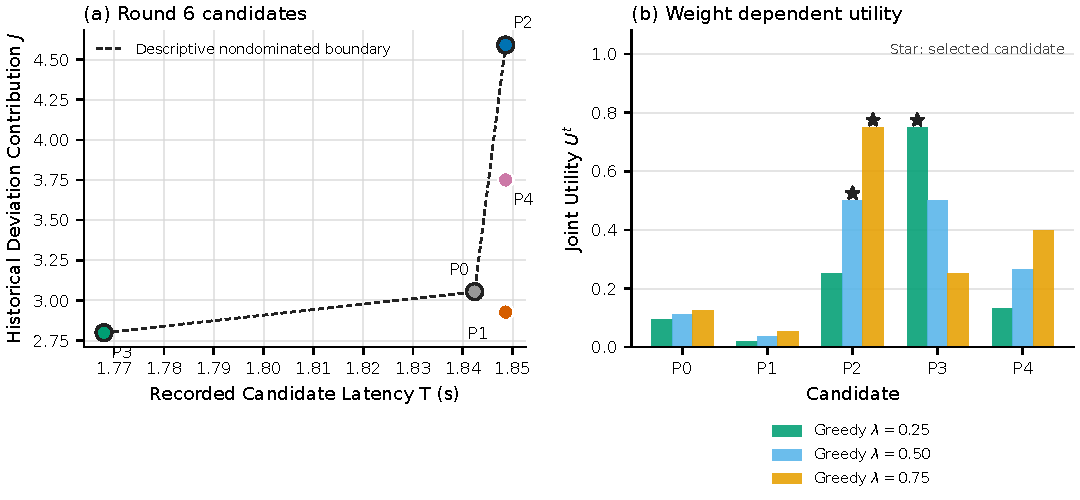
\includegraphics[width=0.98\textwidth]{experiment_J_T_candidate_scores.pdf}
\caption{Candidate scores for the round 6 decision from the common
state after round 5.  Panel (a) shows raw $J$ and
$T_{\mathrm{sys}}$ values and a descriptive nondominated boundary for
larger $J$ and smaller $T$.  Panel (b) shows the joint utility for
three values of $\lambda$; stars mark the selected candidates.  The
boundary is an analysis aid and is not an optimization stage.}
\label{fig:jt_candidate_scores}
\end{figure*}

\textbf{Mode selection and switching.}
Figure~\ref{fig:selection_switching} records the executed candidate in
every round and distinguishes two switching measures.  A candidate
change counts a transition between adjacent candidate names; a client
mode reassignment counts every client whose Mode changes.  Greedy
$\lambda=0.75$ and Maximum $J$ select $P_2$ in all 95 rounds after the
prefix.  Each therefore has one candidate change and 20 client
reassignments, and their complete learning and latency trajectories
coincide.  Greedy $\lambda=0.25$ selects $P_3$ in 93 of the 95
post prefix rounds and has five candidate changes.  Greedy
$\lambda=0.50$ alternates among $P_2$, $P_3$, and $P_4$, producing
52 candidate changes and 1,558 client reassignments.  Hysteresis
reduces these totals to 22 and 649, while periodic selection reduces
them to 14 and 411.

\begin{figure*}[t]
\centering
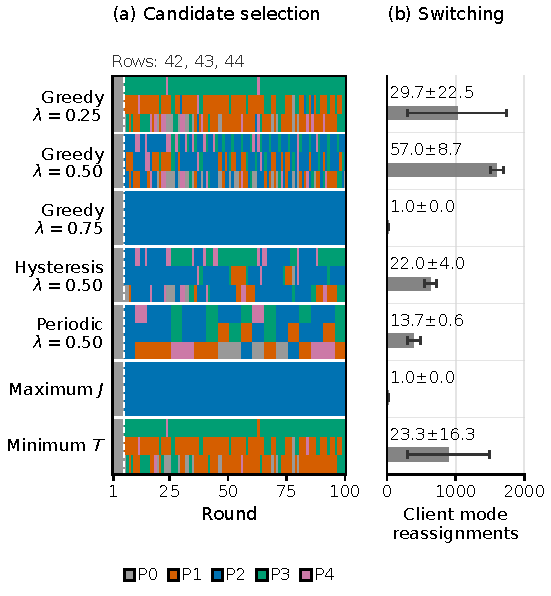
\includegraphics[width=0.98\textwidth]{experiment_selection_switching.pdf}
\caption{Candidate selection and switching behavior for the seven
dynamic strategies in seed 42.  Panel (a) shows the candidate executed
in each round; rounds 1 to 5 form the common $P_0$ prefix.  Panel (b)
reports total client mode reassignments, with adjacent candidate
changes printed beside each bar.}
\label{fig:selection_switching}
\end{figure*}

These records establish that $J^t(\mathbf h^t)$ is operationally
active in the selector: increasing $\lambda$ changes the candidate,
and the largest weight reproduces the Maximum $J$ policy in this run.
They do not establish that a larger value of $J$ causes a lower test
loss.  Candidate $P_2$ assigns half of the clients to $FL_{EC}$ and
therefore also changes training work, communication, and the
subsequent model and history states.  These factors cannot be
separated by the observed trajectory alone.

\subsection{Discussion and Limitations}
\label{sec:experiment_limits}

Within the complete seed 42 matrix, the observed operating points show
an empirical tradeoff.  A low weight on $J$ favors the faster $P_3$
profile, while a high weight favors the stronger historical deviation
contribution of $P_2$.  The latter choice increases local work and
communication, but its final loss remains competitive with the best
fixed mixed candidate, Fixed $P_2$.
This evidence supports the narrower statement that joint selection
can retain candidates with a stronger historical deviation signal
under an explicit system latency preference.  It does not support the
claim that a larger $J$ necessarily improves optimization or test
performance.

Several limits qualify the result.  First, only seed 42 provides the
complete fifteen strategy matrix at the analysis snapshot; the
incomplete additional seeds are not used for uncertainty estimates.
Second, the experiment covers Fashion MNIST, one topology, and one
range of synthetic computation and network heterogeneity.  Third,
the latency values come from an event simulator without shared link
contention or a physical deployment.  Fourth, fixed strategies and
dynamic strategies do not all share the same first five rounds, so
small differences such as those between Fixed $P_2$ and Greedy
$\lambda=0.75$ cannot be attributed solely to switching.  Fifth, the
treatment of the asynchronous $FL_E$ upload differs between the
recorded global barrier and the current text of
Eq.~\eqref{eq:system_round_latency}; that definition must be reconciled
before claiming exact formula level validation for $FL_E$ latency.
Finally, the included files pass the structural checks used to build
the figures, but their stored campaign status still marks the separate
independent audit as pending.

\FloatBarrier


\section{Conclusion}
\label{sec:conclusion}
This paper presented a dynamic cloud-edge-end collaboration reconfiguration
framework for federated learning under resource and privacy constraints. The
unified collaboration space represents execution placement, aggregation
topology, transmitted objects, and return paths as the dynamic decision, while a
mode-specific exposure contract determines where DP and HE are required. The
joint model evaluates latency, communication, candidate-specific DP distortion,
encrypted aggregation overhead, and estimated convergence error cost. The constrained multiobjective formulation is solved by bounded Pareto
search and ideal point Tchebycheff selection.

The current framework uses profiled computation and link rates in its logical
latency model, while the training process and CKKS aggregation are executed on
one host. Future work will combine online profiling with physical
cloud-edge-end deployment and will further reduce reconfiguration overhead
through parallel profile evaluation, distributed search, and warm starts.

\appendix
\bibliographystyle{elsarticle-num}
\bibliography{refs}

\end{document}
